\section{Austrian Grand prix}

\subsection{Circuit Analysis}

\textbf{Circuit Name:} Red Bull Ring (Spielberg, Austria) \\
\textbf{Length:} 4.318 km - \textbf{Laps:} 71 - \textbf{Total Distance:} 306.452 km

\begin{figure}[H]
    \centering
    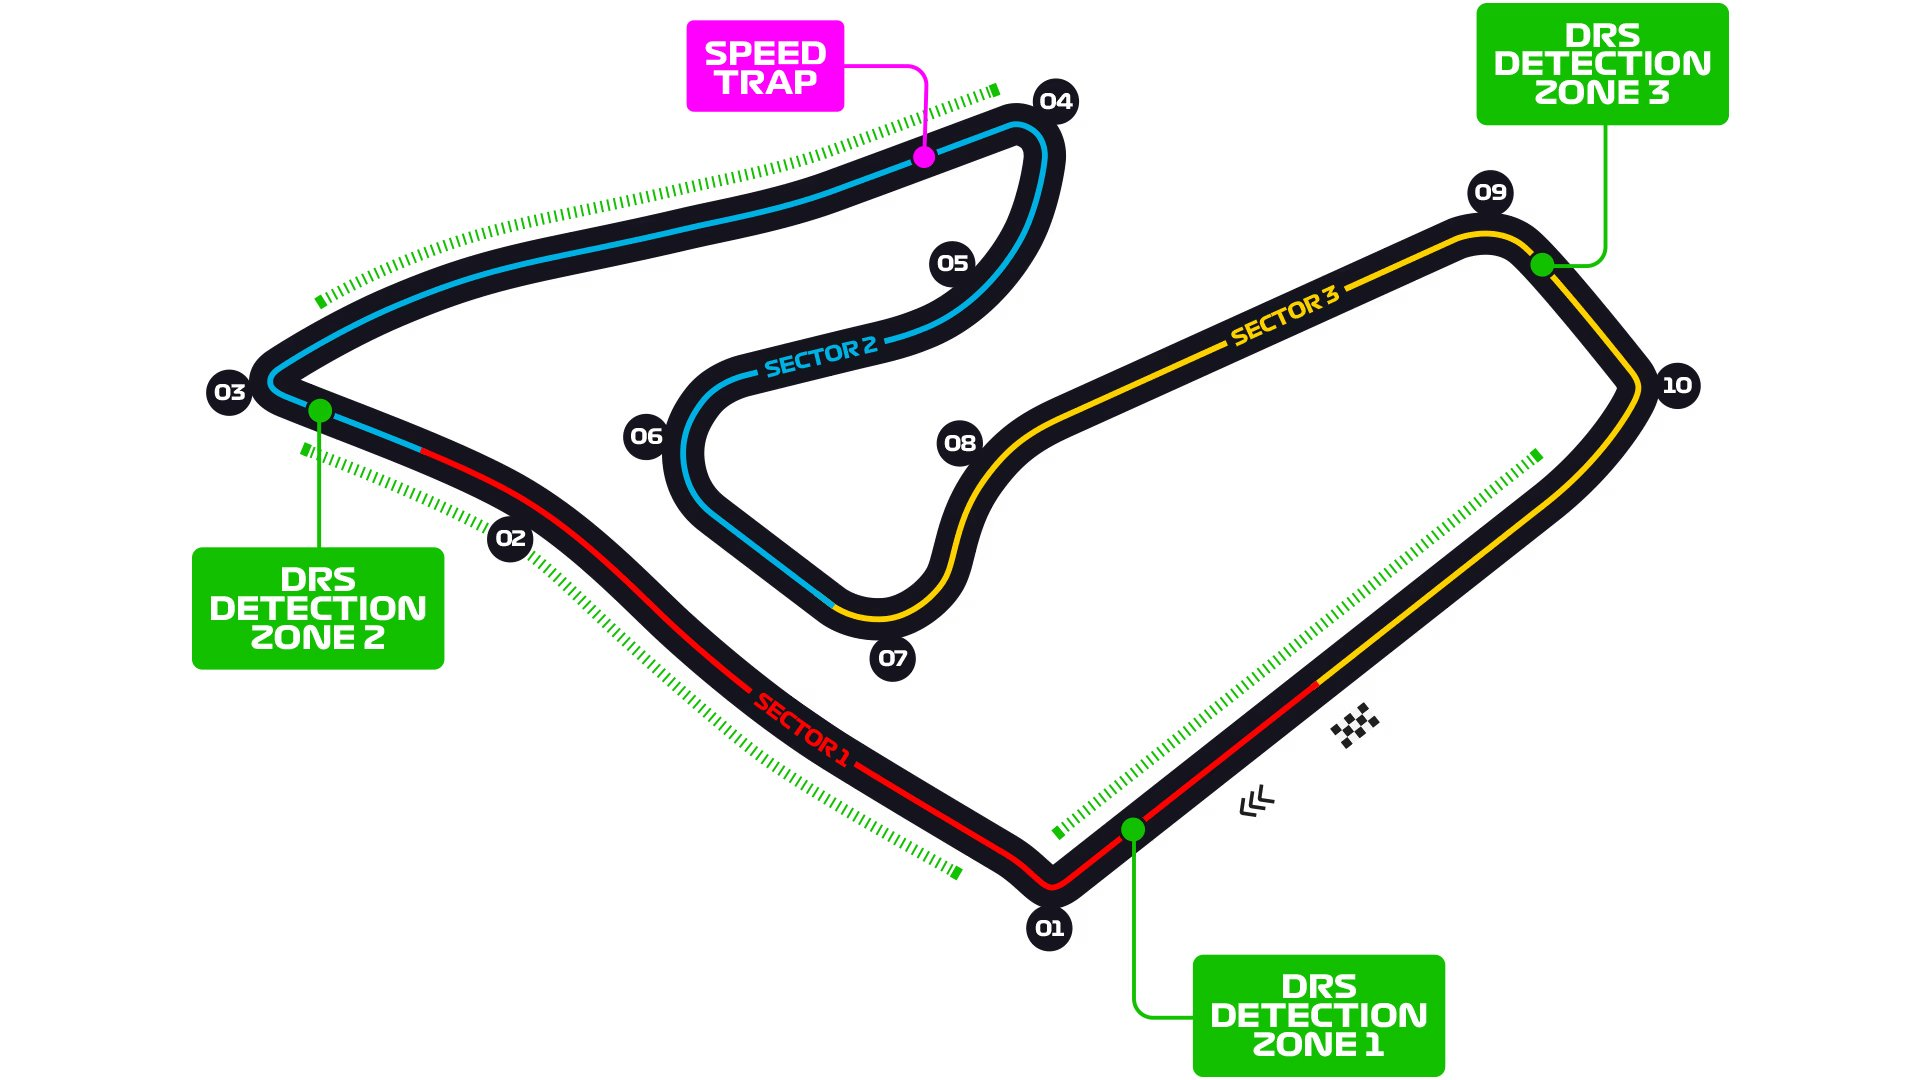
\includegraphics[width=0.75\linewidth]{images/11.Austria_Circuit.jpg}
\end{figure}

\begin{itemize}
    \item \textbf{Lap Record} : 1:02.939 (2020, Valtteri Bottas – Mercedes).
    
    \item \textbf{Number of Corners \& Key Features} : 10 turns (7 right, 3 left) - Short, fast lap with big elevation changes. Mix of long straights and heavy braking zones.
    
    \item \textbf{Braking Zones \& Traction} : Three heavy braking zones at Turns 1, 3, and 4. Strong traction out of slow corners critical to lap time and overtaking.

    \item \textbf{DRS \& Overtaking} : Three DRS zones (main straight, before Turn 3, before Turn 4). \\
    Overtaking opportunities primarily at Turns 3 and 4.
    
    \item \textbf{Tyre Degradation \& Strategy} : Track is usually low degradation but traction zones stress rear tyres.\\
    Two-stop strategies common, but one-stop sometimes possible with tyre management.
    
    \item \textbf{Weather \& Environment} : Mountain climate can bring sudden rain.\\
    High altitude reduces downforce and engine power, favouring efficient aero packages.
\end{itemize}

\textbf{Strategic Summary :}
The Red Bull Ring rewards cars with straight-line speed, strong braking, and traction. Short lap amplifies traffic management in qualifying and strategy timing during the race.


\subsection{Race Analysis}

\textbf{Date:} Sprint : 29 June 2024 - 12:00 local time\\
Race : 30 June 2024 — 15:00 local time 

\begin{itemize}
    \item \textbf{Sprint Qualifying:} \textbf{Pole Position:} Max Verstappen (Red Bull) – 1:04.686.\\
    Grid : Norris 2nd, Piastri 3rd, Russell 4th.

    \item \textbf{Sprint Summary} : \textbf{Winner:} Max Verstappen (Red Bull). \\
    \textbf{Podium}: 1. Verstappen - 2. Piastri - 3. Norris. \\
    Norris briefly overtook Verstappen into Turn 3 but was repassed; Piastri also attacked but couldn’t convert.
    
    \item \textbf{Qualifying Summary} : \textbf{Pole Position:} Max Verstappen (Red Bull) – 1:04.314. \\
    Grid: Norris 2nd, Russell 3rd, Sainz 4th.
    
    \item \textbf{Race Summary} : \textbf{Winner:} George Russell (Mercedes).\\
    \textbf{Podium:} 1. Russell - 2. Piastri - 3. Sainz.\\
    \textbf{Notable incidents:} Verstappen–Norris collision at Turn 3, 6 laps before the end (Virtual Safety Car deployed late after).
    
    \item \textbf{Strategies} : Most teams on two-stop strategies (Medium–Hard–Medium).\\
    - Verstappen and Norris ran aggressive stints, pushing hard early, leading to tyre wear and tension in final laps. \\
    - Russell and Mercedes opted for a conservative but well-executed Medium–Hard–Hard, staying in contention. \\
    - Piastri extended his middle stint, allowing fresher tyres to overtake Sainz late for P2. \\
    - Ferrari mirrored McLaren but couldn’t match pace. Leclerc lost out with traffic and track limits, finishing P11.\\
    - Haas split strategies: both Hülkenberg and Magnussen scored strong points with consistent tyre management.
    
    \item \textbf{Performance Trends} : \textbf{Mercedes:} Opportunistic and precise. Russell’s consistency brought first win since Brazil 2022. Hamilton solid P4 despite a 5s penalty. \\
    \textbf{McLaren:} Fastest car overall, but Norris’s clash wasted a possible win. Piastri salvaged superb P2. \\
    \textbf{Red Bull:} Verstappen dominant until collision, Pérez mediocre (P7). First cracks in home dominance. \\
    \textbf{Ferrari:} Sainz consistent P3; Leclerc struggled with pace and penalties, finishing out of points. \\
    \textbf{Haas:} Standout of midfield — double points (Hülkenberg P6, Magnussen P8).
    
    \item \textbf{Championship Impact} : \textbf{Drivers:} Verstappen 237 points, Norris 156, Leclerc 150.\\
    \textbf{Constructors:} Red Bull 355, Ferrari 291, McLaren 268, Mercedes 196.    
\end{itemize}

\textbf{Key Takeaway :}
The Verstappen–Norris clash opened the door for Russell and Mercedes. McLaren again showed genuine race-winning speed, while Ferrari continued consistent podium scoring. Red Bull’s dominance cracked under pressure at their home race.


\subsection{Link \& Takeaway}

\begin{itemize}
    \item The Red Bull Ring’s heavy braking zones and traction battles suited Red Bull and McLaren, explaining their duel at the front. 
    \item Mercedes capitalised perfectly when fortune turned, confirming progress. 
    \item Ferrari again lacked the ultimate pace but benefited from rivals’ misfortune.
    \item Haas delivered their best weekend in years, while Aston Martin continued to decline.
\end{itemize}